\documentclass[12pt]{extarticle}
\usepackage{phys440}

\title{PHYS440 - Exercises from Wong 2022}
\author{John Hurst}
\date{November 2023}

\begin{document}
\maketitle

%%%%%%%%%%%%%%%%%%%%%%%%%%%%%%%%%%%%%%%%%%%%%%%%%%%%%%%%%%%%%%%%%%%%%%%%%%%%%%%%%%%%%%%%%%%%%%%%%%%%
\question{1.1}{How many possible states do (a) four coins have? (b) five coins?
}

Four coins have $2^4=16$ possible states.
Five coins have $2^5=32$ possible states.

%%%%%%%%%%%%%%%%%%%%%%%%%%%%%%%%%%%%%%%%%%%%%%%%%%%%%%%%%%%%%%%%%%%%%%%%%%%%%%%%%%%%%%%%%%%%%%%%%%%%
\question{1.2}{How many possible states do (a) four dice have? (b) five dice?
}

Four dice have $6^4=1296$ possible states.
Five dice have $6^5=7776$ possible states.

%%%%%%%%%%%%%%%%%%%%%%%%%%%%%%%%%%%%%%%%%%%%%%%%%%%%%%%%%%%%%%%%%%%%%%%%%%%%%%%%%%%%%%%%%%%%%%%%%%%%
\question{1.3}{Some board games use a twenty-sided die. How many twenty-sided dice does it take to code the seven colors of the rainbow?
}

Seven colors can be encoded with a single twenty-sided die, because $7<20$.

%%%%%%%%%%%%%%%%%%%%%%%%%%%%%%%%%%%%%%%%%%%%%%%%%%%%%%%%%%%%%%%%%%%%%%%%%%%%%%%%%%%%%%%%%%%%%%%%%%%%
\question{1.4}{How many (a) coins and (b) six-sided dice would it take to represent the 26 letters of the English alphabet?
Ignore upper and lowercase, spaces, punctuation etc, so there's only 26 letters total.
}

26 letters can be encoded with 5 coins, because $2^5=32>26$.
The letters can be encoded with two dice, because $6^2=36>26$.

Another way to compute it is to use the logarithm:
\begin{align*}
\ceil{\log_2{26}} &= 5 \\
\ceil{\log_6{26}} &= 2
\end{align*}

%%%%%%%%%%%%%%%%%%%%%%%%%%%%%%%%%%%%%%%%%%%%%%%%%%%%%%%%%%%%%%%%%%%%%%%%%%%%%%%%%%%%%%%%%%%%%%%%%%%%
\question{1.5}{Convert the following binary (base 2) numbers to decimal numbers (base 10): (a) $10111_2$, (b) $11001010_2$.
}

\begin{align*}
2^4+2^2+2^1+2^0 &= 16+4+2+1 = 23 \\
2^7+2^6+2^3+2^1 &= 128+64+8+2 = 202
\end{align*}

%%%%%%%%%%%%%%%%%%%%%%%%%%%%%%%%%%%%%%%%%%%%%%%%%%%%%%%%%%%%%%%%%%%%%%%%%%%%%%%%%%%%%%%%%%%%%%%%%%%%
\question{1.6}{Convert the following decimal (base 10) numbers to binary numbers (base 2): (a) $42$, (b) $495$.
}

\begin{enumerate}[itemsep=-2mm]
\item Divide 42 by 2: the result is 21, with remainder 0.
\item Divide 21 by 2: the result is 10, with remainder 1.
\item Divide 10 by 2: the result is 5, with remainder 0.
\item Divide 5 by 2: the result is 2, with remainder 1.
\item Divide 2 by 2: the result is 1, with remainder 0.
\item Divide 1 by 2: the result is 0, with remainder 1.
\item The binary number is $101010_2$.
\end{enumerate}

\begin{enumerate}[itemsep=-2mm]
\item Divide 495 by 2: the result is 247, with remainder 1.
\item Divide 247 by 2: the result is 123, with remainder 1.
\item Divide 123 by 2: the result is 61, with remainder 1.
\item Divide 61 by 2: the result is 30, with remainder 1.
\item Divide 30 by 2: the result is 15, with remainder 0.
\item Divide 15 by 2: the result is 7, with remainder 1.
\item Divide 7 by 2: the result is 3, with remainder 1.
\item Divide 3 by 2: the result is 1, with remainder 1.
\item Divide 1 by 2: the result is 0, with remainder 1.
\item The binary number is $111101111_2$.
\end{enumerate}

%%%%%%%%%%%%%%%%%%%%%%%%%%%%%%%%%%%%%%%%%%%%%%%%%%%%%%%%%%%%%%%%%%%%%%%%%%%%%%%%%%%%%%%%%%%%%%%%%%%%
\question{1.7}{Base 16, commonly called hexadecimal, is another frequently used number system in computing. The sixteen digits are 0, 1, 2, 3, 4, 5, 6, 7, 8, 9, A, B, C, D, E, F. So the letter A is ten in decimal, ... and F is fifteen in decimal.
\begin{enumerate}[(a)]
\item Convert the hexadecimal number 3B7C to a decimal (base 10) number.
\item Convert the hexadecimal number FF to a binary (base 2) number. (So two hexadecimal numbers can represent eight bits.)
\item Convert the hexadecimal numbers FA, 10 and E4 to decimal.
\end{enumerate}
}

\begin{enumerate}[(a)]
\item $16^3\times 3 + 16^2\times 11 + 16^1\times 7 + 16^0\times 12 = 15228$.
\item $FF_{16} = 11111111_2$.
\item $16\times 15 + 10 = 250$, $16 + 0 = 16$, $16\times 14 + 4 = 228$.
\end{enumerate}

%%%%%%%%%%%%%%%%%%%%%%%%%%%%%%%%%%%%%%%%%%%%%%%%%%%%%%%%%%%%%%%%%%%%%%%%%%%%%%%%%%%%%%%%%%%%%%%%%%%%
\question{1.8}{Negative numbers can be encoded in binary using \textit{two's complement},
where the most significant bit is negative, while the remaining bits are positive.
Convert each of these two's complement numbers to decimal: 000, 001, 010, 011, 100, 101, 110, 111.
}
\begin{center}
\begin{tabular}{|c|r|}
    \hline
    Binary & Decimal \\
    \hline
    000 & 0 \\
    001 & 1 \\
    010 & 2 \\
    011 & 3 \\
    100 & -4 \\
    101 & -3 \\
    110 & -2 \\
    111 & -1 \\
    \hline
\end{tabular}
\end{center}

%%%%%%%%%%%%%%%%%%%%%%%%%%%%%%%%%%%%%%%%%%%%%%%%%%%%%%%%%%%%%%%%%%%%%%%%%%%%%%%%%%%%%%%%%%%%%%%%%%%%
\question{1.9}{Write your name as an ASCII bit string.
}

\texttt{"John Hurst"} is encoded as
\begin{center}
\begin{tabular}{|c|c|c|}
    \hline
    Character & ASCII & Binary \\
    \hline
    J & 74 & 01001010 \\
    o & 111 & 01101111 \\
    h & 104 & 01101000 \\
    n & 110 & 01101110 \\
    (space) & 32 & 00100000 \\
    H & 72 & 01001000 \\
    u & 117 & 01110101 \\
    r & 114 & 01110010 \\
    s & 115 & 01110011 \\
    t & 116 & 01110100 \\
    \hline
\end{tabular}
\end{center}

%%%%%%%%%%%%%%%%%%%%%%%%%%%%%%%%%%%%%%%%%%%%%%%%%%%%%%%%%%%%%%%%%%%%%%%%%%%%%%%%%%%%%%%%%%%%%%%%%%%%
\question{1.10}{Decode the following ASCII characters: 1010001, 1110101, 1100001, 1101110, 1110100, 1110101, 1101101.
}

\begin{center}
\begin{tabular}{|c|c|c|}
    \hline
    Binary & ASCII & Character \\
    \hline
    01010001 & 81 & Q \\
    01110101 & 117 & u \\
    01100001 & 97 & a \\
    01101110 & 110 & n \\
    01110100 & 116 & t \\
    01110101 & 117 & u \\
    01101101 & 109 & m \\
    \hline
\end{tabular}
\end{center}


%%%%%%%%%%%%%%%%%%%%%%%%%%%%%%%%%%%%%%%%%%%%%%%%%%%%%%%%%%%%%%%%%%%%%%%%%%%%%%%%%%%%%%%%%%%%%%%%%%%%
\question{1.11}{Consider the following gate that inverts the inputs before passing them into an OR gate, sometimes called a \textit{negative-OR gate}:

\begin{center}
\begin{circuitikz}
    \ctikzset{color=blue}
    % NOT gates and an OR gate to represent NOT(A) OR NOT(B)
    \draw
    (0,0) node[not port] (nota) {}
    (0,-2) node[not port] (notb) {}
    (nota.in) node[anchor=east] {A}
    (notb.in) node[anchor=east] {B}
    (3,-1) node[or port] (myor) {}
    (nota.out) -| (myor.in 1)
    (notb.out) -| (myor.in 2)
    (myor.out) node[anchor=west] {NOT(A) OR NOT(B)};
\end{circuitikz}
\end{center}

\begin{enumerate}[(a)]
\item Write the truth table for this circuit.
\item What logic gate is this equivalent to?
\end{enumerate}
}

\begin{enumerate}[(a)]
\item The truth table is:
\begin{center}
\begin{tabular}{|c|c|c|}
    \hline
    A & B & NOT(A) OR NOT(B) \\
    \hline
    0 & 0 & 1 \\
    0 & 1 & 1 \\
    1 & 0 & 1 \\
    1 & 1 & 0 \\
    \hline
\end{tabular}
\end{center}
\item This is equivalent to a NAND gate.
\end{enumerate}

%%%%%%%%%%%%%%%%%%%%%%%%%%%%%%%%%%%%%%%%%%%%%%%%%%%%%%%%%%%%%%%%%%%%%%%%%%%%%%%%%%%%%%%%%%%%%%%%%%%%
\question{1.12}{Consider the following gate that inverts the inputs before passing them into an AND gate, sometimes called a \textit{negative-AND gate}:

\begin{center}
\begin{circuitikz}
    \ctikzset{color=blue}
    % NOT gates and an AND gate to represent NOT(A) AND NOT(B)
    \draw
    (0,0) node[not port] (nota) {}
    (0,-2) node[not port] (notb) {}
    (nota.in) node[anchor=east] {A}
    (notb.in) node[anchor=east] {B}
    (3,-1) node[and port] (myand) {}
    (nota.out) -| (myand.in 1)
    (notb.out) -| (myand.in 2)
    (myand.out) node[anchor=west] {NOT(A) AND NOT(B)};
\end{circuitikz}
\end{center}

\begin{enumerate}[(a)]
\item Write the truth table for this circuit.
\item What logic gate is this equivalent to?
\end{enumerate}
}

\begin{enumerate}[(a)]
\item The truth table is:
\begin{center}
\begin{tabular}{|c|c|c|}
    \hline
    A & B & NOT(A) AND NOT(B) \\
    \hline
    0 & 0 & 1 \\
    0 & 1 & 0 \\
    1 & 0 & 0 \\
    1 & 1 & 0 \\
    \hline
\end{tabular}
\end{center}
\item This is equivalent to a NOR gate.
\end{enumerate}

%%%%%%%%%%%%%%%%%%%%%%%%%%%%%%%%%%%%%%%%%%%%%%%%%%%%%%%%%%%%%%%%%%%%%%%%%%%%%%%%%%%%%%%%%%%%%%%%%%%%
\question{1.13}{Consider the following electrical circuit:

\begin{center}
\begin{circuitikz}
    \ctikzset{color=blue}
    \draw (0,0) to[battery] (0,4); % Battery, vertical
    \draw (3,0) to[spst, l=B] (3,2) % Switch B
                to[spst, l=A] (3,4); % Switch A
    \draw (6,0) to[lamp, l=Output] (6,4); % Lightbulb (lamp) as Output
    \draw (0,4) -- (6,4); % Wire to the parallel path
    \draw (0,0) -- (6,0); % Closing the circuit
\end{circuitikz}
\end{center}

Answer the following questions:
\begin{enumerate}[(a)]
\item Say $A=0$ and $B=0$. Is the light bulb off or on?
\item Say $A=0$ and $B=1$. Is the light bulb off or on?
\item Say $A=1$ and $B=0$. Is the light bulb off or on?
\item Say $A=1$ and $B=1$. Is the light bulb off or on?
\item What logic gate does this circuit correspond to?
\end{enumerate}
}

\begin{enumerate}[(a)]
\item When both switches are off, the current flows through the light bulb, so it is on.
\item When switch $A$ is off, the current flows through the light bulb, so it is on.
\item When switch $B$ is off, the current flows through the light bulb, so it is on.
\item When both switches are on, the current flows through the switches, so the light bulb is off.
\item This circuit corresponds to a NAND gate.
\end{enumerate}

%%%%%%%%%%%%%%%%%%%%%%%%%%%%%%%%%%%%%%%%%%%%%%%%%%%%%%%%%%%%%%%%%%%%%%%%%%%%%%%%%%%%%%%%%%%%%%%%%%%%
\question{1.14}{Consider the following electrical circuit:
\begin{center}
\begin{circuitikz}
    \ctikzset{color=blue}
    \draw (0,4) to[battery] (3,4) -- (6,4); % Battery
    \draw (0,0) -- (6,0);
    \draw (0,0) to [lamp, l=Output] (0,4); % Lightbulb (lamp) as Output
    \draw (3,0) to [spst, l=A] (3,4); % Switch A
    \draw (6,0) to [spst, l=B] (6,4); % Switch B
\end{circuitikz}
\end{center}

Answer the following questions:
\begin{enumerate}[(a)]
\item Say $A=0$ and $B=0$. Is the light bulb off or on?
\item Say $A=0$ and $B=1$. Is the light bulb off or on?
\item Say $A=1$ and $B=0$. Is the light bulb off or on?
\item Say $A=1$ and $B=1$. Is the light bulb off or on?
\item What logic gate does this circuit correspond to?
\end{enumerate}
}

\begin{enumerate}[(a)]
\item When both switches are off, the current does not flow, so the light bulb is off.
\item When switch $A$ is off, and switch $B$ is on, the current flows through switch $B$, so the light bulb is on.
\item When switch $A$ is on, and switch $B$ is off, the current flows through switch $A$, so the light bulb is on.
\item When both switches are on, the current flows through both switches, so the light bulb is on.
\item This circuit corresponds to an OR gate.
\end{enumerate}

%%%%%%%%%%%%%%%%%%%%%%%%%%%%%%%%%%%%%%%%%%%%%%%%%%%%%%%%%%%%%%%%%%%%%%%%%%%%%%%%%%%%%%%%%%%%%%%%%%%%
\question{1.15}{Consider the following electrical circuit:
\begin{center}
\begin{circuitikz}
    \ctikzset{color=blue}
    \draw (0,0) to[battery] (0,4); % Battery, vertical
    \draw (2,0) to [spst, l=A] (2,4); % Switch A
    \draw (4,0) to [spst, l=B] (4,4); % Switch B
    \draw (6,0) to [lamp, l=Output] (6,4); % Lightbulb (lamp) as Output
    \draw (0,0) -- (6,0);
    \draw (0,4) -- (6,4);
\end{circuitikz}
\end{center}

Answer the following questions:
\begin{enumerate}[(a)]
\item Say $A=0$ and $B=0$. Is the light bulb off or on?
\item Say $A=0$ and $B=1$. Is the light bulb off or on?
\item Say $A=1$ and $B=0$. Is the light bulb off or on?
\item Say $A=1$ and $B=1$. Is the light bulb off or on?
\item What logic gate does this circuit correspond to?
\end{enumerate}
}

\begin{enumerate}[(a)]
\item When both switches are off, the current flows through the light bulb, so it is on.
\item When switch $A$ is off and switch $B$ is on, the current flows through switch $B$, so the light bulb is off.
\item When switch $A$ is on and switch $B$ is off, the current flows through switch $A$, so the light bulb is off.
\item When both switches are on, the current flows through both switches, so the light bulb is off.
\item This circuit corresponds to a NOR gate.
\end{enumerate}

%%%%%%%%%%%%%%%%%%%%%%%%%%%%%%%%%%%%%%%%%%%%%%%%%%%%%%%%%%%%%%%%%%%%%%%%%%%%%%%%%%%%%%%%%%%%%%%%%%%%
\question{1.16}{In some homes in the United States, special switches are used so that two switches control a single light.
Often, these switches are located at opposite ends of a stairway or a hallway, and either switch can be used to turn the light on or off.
A traditional switch enables or disables the flow of electricity through a single wire.
In contrast, these special switches, called \textit{three pole switches}, choose between two different wires.
The following electrical circuit gives an example:
\begin{center}
\begin{circuitikz}
    \ctikzset{color=blue}
    \draw
    (0,0) to [battery] (0,2) --
    (1,2) node[spdt] (spdtA) {}
    (4,2) node[spdt,rotate=180] (spdtB) {}
    (0,2) -- (spdtA.in)
    (spdtA.out 1) -- (spdtB.out 1)
    (spdtA.out 2) -- (spdtB.out 2)
    (spdtB.in) -- (5,2)
    (5,2) to [lamp, l=Output] (5,0)
    -- (0,0)
    (spdtA.in) node[below] {C}
    (spdtA.out 1) node[right] {0}
    (spdtA.out 2) node[right] {1}
    (spdtB.out 1) node[left] {1}
    (spdtB.out 2) node[left] {0}
    (spdtB.in) node[above] {C};
    \draw[dashed] (0.25,1.4) rectangle (2.25,2.6);
    \draw[dashed] (2.75,1.4) rectangle (4.75,2.6);
    \node[] at (1,2.9) {Switch A};
    \node[] at (3.5,2.9) {Switch B};
\end{circuitikz}
\end{center}

Each switch has three poles, labeled $C$, 0 and 1.
Switch $A$ is currently flipped up, which connects $C$ and 0.
Switch $B$ is currently flipped down, which connects $C$ and 1.
In this configuration, there is a complete path for the electricty to flow.
It comes out of the positive end of the battery, through Switch $A$ along $A=0$, then down to $B=1$, then through Switch $B$, then down through the light bulb, left through the bottom wire, and up to the negative end of the battery.
So, the light bulb is on when $A=0$ and $B=1$.

\begin{enumerate}[(a)]
\item Say $A=0$ and $B=0$. Is the light bulb off or on?
\item Say $A=1$ and $B=0$. Is the light bulb off or on?
\item Say $A=1$ and $B=1$. Is the light bulb off or on?
\item What logic gate does this circuit correspond to?
\end{enumerate}
}

\begin{enumerate}[(a)]
\item When switch $A$ is up (0) and switch $B$ is up (0), the current does not flow, so the light bulb is off.
\item When switch $A$ is down (1) and switch $B$ is up (0), the current flows through switch $A$ and then switch $B$, so the light bulb is on.
\item When switch $A$ is down (1) and switch $B$ is down (1), the current does not flow, so the light bulb is off.
\item This circuit corresponds to an XOR gate.
\end{enumerate}

%%%%%%%%%%%%%%%%%%%%%%%%%%%%%%%%%%%%%%%%%%%%%%%%%%%%%%%%%%%%%%%%%%%%%%%%%%%%%%%%%%%%%%%%%%%%%%%%%%%%
\question{1.17}{Visit the Wikipedia article ``Transistor count''\cite{wikipedia_transistor_count}.
\begin{enumerate}[(a)]
\item Pick an older computer processor. Which one did you pick, what year was it introduced, and how many transistors did it have?
\item Pick a newer computer processor. Which one did you pick, what year was it introduced, and how many transistors did it have?
\end{enumerate}
}

\begin{enumerate}[(a)]
\item The Zilog Z80 processor was introduced in 1976 and had 8500 transistors.
\item The 11th gen Intel Core processor was introduced in 2021 and has more than 6 billion transistors.
\end{enumerate}


%%%%%%%%%%%%%%%%%%%%%%%%%%%%%%%%%%%%%%%%%%%%%%%%%%%%%%%%%%%%%%%%%%%%%%%%%%%%%%%%%%%%%%%%%%%%%%%%%%%%
\question{2.8}{A qubit is in the state
\[
\frac{e^{i\pi/8}}{\sqrt{5}}\ket{0} + \beta\ket{1}.
\]
What is a possible value of $\beta$?
}
\begin{align*}
\left|\frac{e^{i\pi/8}}{\sqrt{5}}\right|^2 + |\beta|^2 & = 1 \\
\frac{1}{5} + |\beta|^2 & = 1 \\
|\beta|^2 & = \frac{4}{5} \\
|\beta| & = \frac{2}{\sqrt{5}} \\
\beta & = \frac{2e^{i\theta}}{\sqrt{5}}
\end{align*}

%%%%%%%%%%%%%%%%%%%%%%%%%%%%%%%%%%%%%%%%%%%%%%%%%%%%%%%%%%%%%%%%%%%%%%%%%%%%%%%%%%%%%%%%%%%%%%%%%%%%
\question{2.9}{A qubit is in the state
\[
A\left(2e^{i\pi/6}\ket{0} - 3\ket{1}\right).
\]
\begin{enumerate}[(a)]
\item Normalize the state (i.e. find $A$).
\item If you measure the qubit, what is the probability that you get $\ket{0}$?
\item If you measure the qubit, what is the probability that you get $\ket{1}$?
\end{enumerate}
}
\begin{enumerate}[(a)]
\item
\begin{align*}
\left|2Ae^{i\pi/6}\right|^2 + |3A|^2 & = 1 \\
4|A|^2 + 9|A|^2 & = 1 \\
13|A|^2 & = 1 \\
|A|^2 & = \frac{1}{13} \\
|A| & = \frac{1}{\sqrt{13}} \\
A & = \frac{e^{i\theta}}{\sqrt{13}}
\end{align*}
\item The probability of measuring $\ket{0}$ is $|2A|^2 = \frac{4}{13}$.
\item The probability of measuring $\ket{1}$ is $|3A|^2 = \frac{9}{13}$.
\end{enumerate}

%%%%%%%%%%%%%%%%%%%%%%%%%%%%%%%%%%%%%%%%%%%%%%%%%%%%%%%%%%%%%%%%%%%%%%%%%%%%%%%%%%%%%%%%%%%%%%%%%%%%
\question{2.10}{A qubit is in the state
\[
\frac{1}{2}\ket{0} - \frac{\sqrt(3)}{2}\ket{1}.
\]
\begin{enumerate}[(a)]
\item If you measure it in the $Z$-basis $\{\ket{0},\ket{1}\}$, what states can you get and with what probabilities?
\item Write the qubit's state in terms of the $X$-basis $\{\ket{+},\ket{-}\}$.
\item If you measure it in the $X$-basis, what states can you get and with what probabilities?
\end{enumerate}
}
\begin{enumerate}[(a)]
\item The probability of measuring $\ket{0}$ is $\left|\frac{1}{2}\right|^2 = \frac{1}{4}$.
The probability of measuring $\ket{1}$ is $\left|-\frac{\sqrt{3}}{2}\right|^2 = \frac{3}{4}$.
\item The $X$-basis states are $\ket{+} = \istwo(\ket{0} + \ket{1})$ and $\ket{-} = \istwo(\ket{0} - \ket{1})$.
Thus we have:
\begin{align*}
\ket{+} & = \istwo\left(\ket{0}+\ket{1}\right) & \ket{-} & = \istwo\left(\ket{0}-\ket{1}\right) \\
\ket{+} + \ket{-1} & = \sqrt{2}\ket{0} & \ket{0} & = \istwo\left(\ket{+}+\ket{-}\right) \\
\ket{+} - \ket{-1} & = \sqrt{2}\ket{1} & \ket{1} & = \istwo\left(\ket{+}-\ket{-}\right)
\end{align*}
From these we calculate the qubit's state in the $X$-basis:
\begin{align*}
\frac{1}{2}\ket{0} - \frac{\sqrt{3}}{2}\ket{1} & = \frac{1}{2}\left(\istwo\left(\ket{+}+\ket{-}\right)\right) - \frac{\sqrt{3}}{2}\left(\istwo\left(\ket{+}-\ket{-}\right)\right) \\
& = \frac{1}{2\sqrt{2}}\ket{+} + \frac{1}{2\sqrt{2}}\ket{-} - \frac{\sqrt{3}}{2\sqrt{2}}\ket{+} + \frac{\sqrt{3}}{2\sqrt{2}}\ket{-} \\
& = \frac{1-\sqrt{3}}{2\sqrt{2}}\ket{+} + \frac{1+\sqrt{3}}{2\sqrt{2}}\ket{-}
\end{align*}
\item The probability of measuring $\ket{+}$ is $\left|\frac{1-\sqrt{3}}{2\sqrt{2}}\right|^2 = \frac{4-2\sqrt{3}}{8} = \frac{2-\sqrt{3}}{4}$.
The probability of measuring $\ket{-}$ is $\left|\frac{1+\sqrt{3}}{2\sqrt{2}}\right|^2 = \frac{4+2\sqrt{3}}{8} = \frac{2+\sqrt{3}}{4}$.
\end{enumerate}

%%%%%%%%%%%%%%%%%%%%%%%%%%%%%%%%%%%%%%%%%%%%%%%%%%%%%%%%%%%%%%%%%%%%%%%%%%%%%%%%%%%%%%%%%%%%%%%%%%%%
\question{2.11}{The following states are opposite points on the Bloch sphere:
\begin{align*}
\ket{a} & = \frac{\sqrt{3}}{2}\ket{0} + \frac{i}{2}\ket{1} \\
\ket{b} & = \frac{i}{2}\ket{0} + \frac{\sqrt{3}}{2}\ket{1}
\end{align*}
So, we can measure relative to them. Now consider a qubit in the state
\[
\frac{1}{2}\ket{0} - \frac{\sqrt{3}}{2}\ket{1}.
\]
\begin{enumerate}[(a)]
\item Write the qubit's state in terms of $\ket{a}$ and $\ket{b}$.
\item If you measure the qubit in the basis $\{\ket{a},\ket{b}\}$, what states can you get and with what probabilities?
\end{enumerate}
}
\begin{enumerate}[(a)]
\item We can write the qubit's state in terms of $\ket{a}$ and $\ket{b}$ using these expressions for $\ket{0}$ and $\ket{1}$:
\begin{align*}
\ket{0} & = \frac{\sqrt{3}}{2}\ket{a} - \frac{i}{2}\ket{b} & \ket{1} & = -\frac{i}{2}\ket{a} + \frac{\sqrt{3}}{2}\ket{b}
\end{align*}
Then:
\begin{align*}
\frac{1}{2}\ket{0} - \frac{\sqrt{3}}{2}\ket{1} & = \frac{1}{2}\left(\frac{\sqrt{3}}{2}\ket{a} - \frac{i}{2}\ket{b}\right) - \frac{\sqrt{3}}{2}\left(-\frac{i}{2}\ket{a} + \frac{\sqrt{3}}{2}\ket{b}\right) \\
& = \frac{\sqrt{3}}{4}\ket{a} - \frac{i}{4}\ket{b} + \frac{i\sqrt{3}}{4}\ket{a} - \frac{3}{4}\ket{b} \\
& = \frac{\sqrt{3}(1+i)}{4}\ket{a} - \frac{3+i}{4}\ket{b} \\
\end{align*}
\item The probability of measuring $\ket{a}$ is $\left|\frac{\sqrt{3}(1+i)}{4}\right|^2 = \frac{3\times (1+1)}{16} = \frac{3}{8}$.
The probability of measuring $\ket{b}$ is $\left|-\frac{3+i}{4}\right|^2 = \frac{1+9}{16} = \frac{5}{8}$.
\end{enumerate}

%%%%%%%%%%%%%%%%%%%%%%%%%%%%%%%%%%%%%%%%%%%%%%%%%%%%%%%%%%%%%%%%%%%%%%%%%%%%%%%%%%%%%%%%%%%%%%%%%%%%
\question{2.12}{A qubit is in the state $\ket{0}$.
If you measure it in the $X$-basis ($\{\ket{+},\ket{-}\}$), and then measure it again in the $Z$-basis ($\{\ket{0},\ket{1}\}$), what is the probability of getting
\begin{enumerate}[(a)]
\item $\ket{0}$?
\item $\ket{1}$?
\end{enumerate}
}

After measuring in the $X$-basis, the qubit is in the state $\ket{+}$ or $\ket{-}$.
From either of these states, a measurement in the $Z$-basis will give
\begin{enumerate}[(a)]
\item $P(\ket{0})=\frac{1}{2}$
\item $P(\ket{1})=\frac{1}{2}$.
\end{enumerate}

%%%%%%%%%%%%%%%%%%%%%%%%%%%%%%%%%%%%%%%%%%%%%%%%%%%%%%%%%%%%%%%%%%%%%%%%%%%%%%%%%%%%%%%%%%%%%%%%%%%%
\question{2.13}{Is there a measurement that can distinguish the following pairs of states?
If yes, give a measurement.
If no, explain your reasoning.
\begin{enumerate}[(a)]
\item $\ket{+} = \istwo(\ket{0}+\ket{1})$ and $e^{i\pi/8}\ket{+} = \frac{e^{i\pi/8}}{\sqrt{2}}(\ket{0}+\ket{1})$
\item $\ket{+} = \istwo(\ket{0}+\ket{1})$ and $\ket{-} = \istwo(\ket{0}-\ket{1})$
\item $\ket{0}$ and $e^{i\pi/4}\ket{0}$
\end{enumerate}
}

\begin{enumerate}[(a)]
\item These states cannot be distinguished, because they differ only by a global phase.
\item These states can be distinguished by measuring in the $X$-basis ($\{\ket{+},\ket{-}\}$).
\item These states cannot be distinguished, because they differ only by a global phase.
\end{enumerate}

%%%%%%%%%%%%%%%%%%%%%%%%%%%%%%%%%%%%%%%%%%%%%%%%%%%%%%%%%%%%%%%%%%%%%%%%%%%%%%%%%%%%%%%%%%%%%%%%%%%%
\question{2.14}{A qubit is in the state
\[
\ket{i} = \istwo(\ket{0}+i\ket{1}).
\]
\begin{enumerate}[(a)]
\item Where on the Bloch sphere is this state? Give your answer in $(\theta,\phi)$ coordinates.
\item Sketch the point on the Bloch sphere.
\end{enumerate}
}

\begin{enumerate}[(a)]
\item
\begin{align*}
\ket{i} & = \istwo\left(\ket{0}+i\ket{1}\right) \\
& = \cos(\frac{\theta}{2})\ket{0} + e^{i\phi}\sin(\frac{\theta}{2})\ket{1} \\
\implies \cos(\frac{\theta}{2}) & = \istwo \\
\frac{\theta}{2} & = \frac{\pi}{4} \\
\theta & = \frac{\pi}{2} \\
e^{i\phi} & = i \\
\phi & = \frac{\pi}{2}
\end{align*}
\item
\begin{figure}[h]
\centering
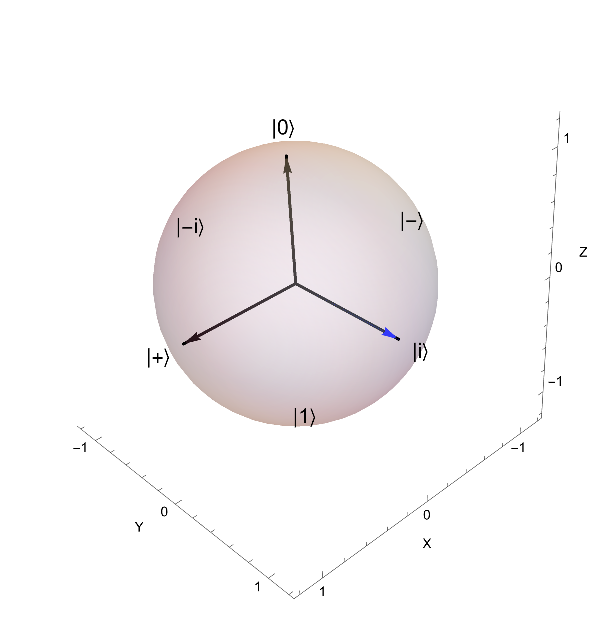
\includegraphics[width=0.5\textwidth]{Exercise2.14-Bloch.eps}
\caption{The point on the Bloch sphere.}
\label{fig:bloch_sphere2.14}
\end{figure}
\end{enumerate}

%%%%%%%%%%%%%%%%%%%%%%%%%%%%%%%%%%%%%%%%%%%%%%%%%%%%%%%%%%%%%%%%%%%%%%%%%%%%%%%%%%%%%%%%%%%%%%%%%%%%
\question{2.15}{A qubit is in the state
\[
\frac{1-i}{2\sqrt{2}}\ket{0} + \frac{\sqrt{3}}{2}\ket{1}.
\]
\begin{enumerate}[(a)]
\item Where on the Bloch sphere is this state? Give your answer in $(\theta,\phi)$ coordinates.
\item Sketch the point on the Bloch sphere.
\end{enumerate}
}

\begin{enumerate}[(a)]
\item
\begin{align*}
\frac{1-i}{2\sqrt{2}}\ket{0} + \frac{\sqrt{3}}{2}\ket{1} & = \frac{e^{7\pi i/4}}{2}\ket{0} + \frac{\sqrt{3}}{2}\ket{1} \\
& \equiv \frac{1}{2}\ket{0} + \frac{e^{-7i\pi/4}\sqrt{3}}{2}\ket{1} \\
\end{align*}
So:
\begin{align*}
\frac{1}{2}\ket{0} + \frac{e^{-7i\pi/4}\sqrt{3}}{2}\ket{1} & = \cos(\frac{\theta}{2})\ket{0} + e^{i\phi}\sin(\frac{\theta}{2})\ket{1} \\
\implies \cos(\frac{\theta}{2}) & = \frac{1}{2} \\
\frac{\theta}{2} & = \frac{\pi}{3} \\
\theta & = \frac{2\pi}{3} \\
e^{i\phi} & = e^{-7i\pi/4} \\
& = e^{i\pi/4} \\
\phi = \frac{\pi}{4}
\end{align*}
\item
\begin{figure}[h]
\centering
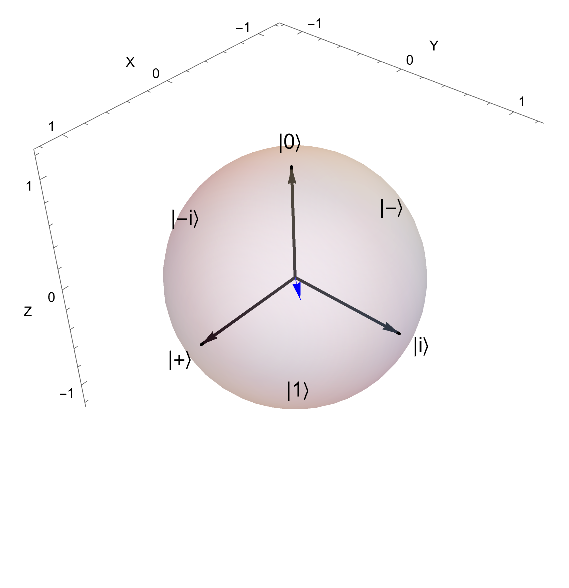
\includegraphics[width=0.5\textwidth]{Exercise2.15-Bloch.eps}
\caption{The point on the Bloch sphere.}
\label{fig:bloch_sphere2.15}
\end{figure}
\end{enumerate}


%%%%%%%%%%%%%%%%%%%%%%%%%%%%%%%%%%%%%%%%%%%%%%%%%%%%%%%%%%%%%%%%%%%%%%%%%%%%%%%%%%%%%%%%%%%%%%%%%%%%
\question{2.16}{Consider the following two states from Exercise 2.11:
\begin{align*}
\ket{a} & = \frac{\sqrt{3}}{2}\ket{0} + \frac{i}{2}\ket{1} \\
\ket{b} & = \frac{i}{2}\ket{0} + \frac{\sqrt{3}}{2}\ket{1}
\end{align*}
Prove that these are opposite points of the Bloch sphere by finding their points in spherical coordinates
$(\theta_a, \phi_a)$ and $(\theta_b, \phi_b)$.
Verify that $\theta_b = \pi - \theta_a$ and $\phi_b = \phi_a + \pi$,
which means they lie on opposite points of the Bloch sphere.
}

\begin{align*}
\ket{a} & = \frac{\sqrt{3}}{2}\ket{0} + \frac{i}{2}\ket{1} \\
& = \cos{\frac{\theta_a}{2}}\ket{0} + e^{i\phi_a}\sin{\frac{\theta_a}{2}}\ket{1} \\
\implies \cos{\frac{\theta_a}{2}} & = \frac{\sqrt{3}}{2} \\
\frac{\theta_a}{2} & = \frac{\pi}{6} \\
\theta_a & = \frac{\pi}{3} \\
e^{i\phi_a} & = i \\
\phi_a & = \frac{\pi}{2} \\
\ket{b} & = \frac{i}{2}\ket{0} + \frac{\sqrt{3}}{2}\ket{1} \\
& = \frac{e^{i\pi/2}}{2}\ket{0} + \frac{\sqrt{3}}{2}\ket{1} \\
& \equiv \frac{1}{2}\ket{0} + \frac{e^{-i\pi/2}\sqrt{3}}{2}\ket{1} \\
& = \frac{1}{2}\ket{0} + \frac{e^{3i\pi/2}\sqrt{3}}{2}\ket{1} \\
& = \cos{\frac{\theta_b}{2}}\ket{0} + e^{i\phi_b}\sin{\frac{\theta_b}{2}}\ket{1} \\
\implies \cos{\frac{\theta_b}{2}} & = \frac{1}{2} \\
\frac{\theta_b}{2} & = \frac{\pi}{3} \\
\theta_b & = \frac{2\pi}{3} \\
e^{i\phi_b} & = e^{3i\pi/2} \\
\phi_b & = \frac{3\pi}{2} \\
\end{align*}

So:
\begin{align*}
\theta_b & = \frac{2\pi}{3} = \pi - \frac{\pi}{3} = \pi - \theta_a \\
\phi_b & = \frac{3\pi}{2} = \frac{\pi}{2} + \pi = \phi_a + \pi
\end{align*}

\todo{Check answer; apparently something wrong with $\phi_a$, $\phi_b$.}


%%%%%%%%%%%%%%%%%%%%%%%%%%%%%%%%%%%%%%%%%%%%%%%%%%%%%%%%%%%%%%%%%%%%%%%%%%%%%%%%%%%%%%%%%%%%%%%%%%%%
\question{2.22}{Consider a map $U$ that transforms the $Z$-basis states as follows:
\begin{align*}
U\ket{0} & = \ket{0}+\ket{1}, \\
U\ket{1} & = \ket{0}-\ket{1}.
\end{align*}
Say $\ket{\psi} = \alpha\ket{0} + \beta\ket{1}$ is a normalized quantum state, i.e. $|\alpha|^2 + |\beta|^2 = 1$.
\begin{enumerate}[(a)]
\item Calculate $U\ket{\psi}$.
\item From your answer to (a), is $U$ a valid quantum gate? Explain your reasoning.
\end{enumerate}
}
\begin{enumerate}[(a)]
\item $U\ket{\psi} = (\alpha+\beta)\ket{0} + (\alpha-\beta)\ket{1}$.
\item $U$ is not a valid quantum gate, because it does not preserve the normalization of the state.
\end{enumerate}

%%%%%%%%%%%%%%%%%%%%%%%%%%%%%%%%%%%%%%%%%%%%%%%%%%%%%%%%%%%%%%%%%%%%%%%%%%%%%%%%%%%%%%%%%%%%%%%%%%%%
\question{2.23}{Consider a map $U$ that transforms the $Z$-basis states as follows:
\begin{align*}
U\ket{0} & = \frac{\sqrt{3}}{2}\ket{0} + \frac{\sqrt{3}+i}{4}\ket{1}, \\
U\ket{1} & = \frac{\sqrt{3}+i}{4}\ket{0} - \frac{\sqrt{3}+3i}{4}\ket{1}.
\end{align*}
Say $\ket{\psi} = \alpha\ket{0} + \beta\ket{1}$ is a normalized quantum state, i.e. $|\alpha|^2 + |\beta|^2 = 1$.
\begin{enumerate}[(a)]
\item Calculate $U\ket{\psi}$.
\item From your answer to (a), is $U$ a valid quantum gate? Explain your reasoning.
\end{enumerate}
}
\begin{enumerate}[(a)]
\item $U\ket{\psi} = \left(\frac{\sqrt{3}}{2}\alpha + \frac{\sqrt{3}+i}{4}\beta\right)\ket{0} + \left(\frac{\sqrt{3}+i}{4}\alpha - \frac{\sqrt{3}+3i}{4}\beta\right)\ket{1}$.
\item $U$ is a valid quantum gate, because $UU^\dagger = I$.
\end{enumerate}


%%%%%%%%%%%%%%%%%%%%%%%%%%%%%%%%%%%%%%%%%%%%%%%%%%%%%%%%%%%%%%%%%%%%%%%%%%%%%%%%%%%%%%%%%%%%%%%%%%%%
\question{4.3}{Calculate the following inner products:
\begin{enumerate}[(a)]
\item $\innerproduct{10}{11}$.
\item $\innerproduct{+-}{01}$.
\item $\innerproduct{1+0}{1-0}$.
\end{enumerate}
}
\begin{enumerate}[(a)]
\item
\begin{align*}
\innerproduct{10}{11} & = \innerproduct{1}{1}\innerproduct{0}{1} \\
& = 1\times 0 \\
& = 0
\end{align*}
This is expected because $\ket{10}$ and $\ket{11}$ are orthogonal.
\item
\begin{align*}
\innerproduct{+-}{01} & = \innerproduct{+}{0}\innerproduct{-}{1} \\
& = \left(\istwo\innerproduct{0}{0} + \istwo\innerproduct{1}{0}\right) \left(\istwo\innerproduct{0}{1} - \istwo\innerproduct{1}{1}\right) \\
& = \left(\istwo\times 1 + \istwo\times 0\right) \left(\istwo\times 0 - \istwo\times 1\right) \\
& = -\frac{1}{2}
\end{align*}

\item
\begin{align*}
\innerproduct{1+0}{1-0} & = \innerproduct{1}{1} \innerproduct{+}{-} \innerproduct{0}{0} \\
& = 1 \times 0 \times 1 \\
& = 0
\end{align*}
\end{enumerate}

%%%%%%%%%%%%%%%%%%%%%%%%%%%%%%%%%%%%%%%%%%%%%%%%%%%%%%%%%%%%%%%%%%%%%%%%%%%%%%%%%%%%%%%%%%%%%%%%%%%%
\question{4.4}{Verify that
\[
\ket{1} \otimes \ket{1} \otimes \ket{0} =
\begin{pmatrix} 0 \\ 0 \\ 0 \\ 0 \\ 0 \\ 0 \\ 1 \\ 0 \end{pmatrix}.
\]
}
\begin{align*}
\ket{1} \otimes \ket{1} \otimes \ket{0} & = \begin{pmatrix} 0 \\ 1 \end{pmatrix} \otimes \begin{pmatrix} 0 \\ 1 \end{pmatrix} \otimes \begin{pmatrix} 1 \\ 0 \end{pmatrix} \\
& = \begin{pmatrix} 0 \\ 1 \end{pmatrix} \otimes \begin{pmatrix} 0 \begin{pmatrix} 1 \\ 0 \end{pmatrix} \\ 1 \begin{pmatrix} 1 \\ 0 \end{pmatrix} \end{pmatrix} \\
& = \begin{pmatrix} 0 \\ 1 \end{pmatrix} \otimes \begin{pmatrix} 0 \\ 0 \\ 1 \\ 0 \end{pmatrix} \\
& = \begin{pmatrix} 0 \begin{pmatrix} 0 \\ 0 \\ 1 \\ 0 \end{pmatrix} \\ 1 \begin{pmatrix} 0 \\ 0 \\ 1 \\ 0 \end{pmatrix} \end{pmatrix} \\
& = \begin{pmatrix} 0 \\ 0 \\ 0 \\ 0 \\ 0 \\ 0 \\ 1 \\ 0 \end{pmatrix}.
\end{align*}

%%%%%%%%%%%%%%%%%%%%%%%%%%%%%%%%%%%%%%%%%%%%%%%%%%%%%%%%%%%%%%%%%%%%%%%%%%%%%%%%%%%%%%%%%%%%%%%%%%%%
\question{4.5}{Consider a two-qubit state
\[
\ket{\psi} = \frac{1}{2}\ket{00} + \frac{i}{\sqrt{2}}\ket{10} + \frac{\sqrt{3}+i}{4}\ket{11}.
\]
\begin{enumerate}[(a)]
\item What is $\ket{\psi}$ as a (column) vector?
\item What is $\bra{\psi}$ as a (row) vector?
\end{enumerate}
}

\begin{enumerate}[(a)]
\item
\[
\ket{\psi} = \begin{pmatrix} \frac{1}{2} \\ 0 \\ \frac{i}{\sqrt{2}} \\ \frac{\sqrt{3}+i}{4} \end{pmatrix}.
\]

\item
\[
\bra{\psi} = \begin{pmatrix} \frac{1}{2} & 0 & -\frac{i}{\sqrt{2}} & \frac{\sqrt{3}-i}{4} \end{pmatrix}.
\]
\end{enumerate}

%%%%%%%%%%%%%%%%%%%%%%%%%%%%%%%%%%%%%%%%%%%%%%%%%%%%%%%%%%%%%%%%%%%%%%%%%%%%%%%%%%%%%%%%%%%%%%%%%%%%
\question{4.6}{Show that $\{\ket{00},\ket{01},\ket{10},\ket{11}\}$ is a complete orthonornmal basis the state of two qubits by showing that it satisfies the completeness relation
\[
\ket{00}\bra{00} + \ket{01}\bra{01} + \ket{10}\bra{10} + \ket{11}\bra{11} = I.
\]
where $I$ is the identity matrix:
\[
I = \begin{pmatrix} 1 & 0 & 0 & 0 \\ 0 & 1 & 0 & 0 \\ 0 & 0 & 1 & 0 \\ 0 & 0 & 0 & 1 \end{pmatrix}.
\]
}
\begin{multline*}
\ket{00}\bra{00} + \ket{01}\bra{01} + \ket{10}\bra{10} + \ket{11}\bra{11} \\
= \begin{pmatrix} 1 \\ 0 \\ 0 \\ 0 \end{pmatrix}\begin{pmatrix} 1 & 0 & 0 & 0 \end{pmatrix} + \begin{pmatrix} 0 \\ 1 \\ 0 \\ 0 \end{pmatrix}\begin{pmatrix} 0 & 1 & 0 & 0 \end{pmatrix} + \begin{pmatrix} 0 \\ 0 \\ 1 \\ 0 \end{pmatrix}\begin{pmatrix} 0 & 0 & 1 & 0 \end{pmatrix} + \begin{pmatrix} 0 \\ 0 \\ 0 \\ 1 \end{pmatrix}\begin{pmatrix} 0 & 0 & 0 & 1 \end{pmatrix} \\
= \begin{pmatrix} 1 & 0 & 0 & 0 \\ 0 & 0 & 0 & 0 \\ 0 & 0 & 0 & 0 \\ 0 & 0 & 0 & 0 \end{pmatrix} + \begin{pmatrix} 0 & 0 & 0 & 0 \\ 0 & 1 & 0 & 0 \\ 0 & 0 & 0 & 0 \\ 0 & 0 & 0 & 0 \end{pmatrix} + \begin{pmatrix} 0 & 0 & 0 & 0 \\ 0 & 0 & 0 & 0 \\ 0 & 0 & 1 & 0 \\ 0 & 0 & 0 & 0 \end{pmatrix} + \begin{pmatrix} 0 & 0 & 0 & 0 \\ 0 & 0 & 0 & 0 \\ 0 & 0 & 0 & 0 \\ 0 & 0 & 0 & 1 \end{pmatrix} \\
= \begin{pmatrix} 1 & 0 & 0 & 0 \\ 0 & 1 & 0 & 0 \\ 0 & 0 & 1 & 0 \\ 0 & 0 & 0 & 1 \end{pmatrix} \\
\end{multline*}

\printbibliography
% \addcontentsline{toc}{section}{References}

\end{document}
